\section{Iteration 6: Decomposition of the Anomaly Detection Unit}
\label{add:it6}

\subsection{Step 1: Identify candidate drivers}
\label{add:it6/drivers}

\npar This iteration is driven by P2': Anomaly detection. The description states
that the load should be balanced ower multiple instances of each subsystem.

\subsection{Step 2: Choose design concepts}
\label{add:it6/concepts}

\npar In this section there will be an overview of the chosen tactics and
patterns.

\subsubsection{Tactics}
\label{add:it6/tactics}

\npar Because anomaly detection algorithms are complicated calculations on large
datasets, it is inherently slow. One simply cannot wait until this process is
completed. Therefore, parallellism is introduced as a tactic. 

\npar This tactic calls for multiple instances but there will not be an infinite
number of resources. Some resource arbitration should be put in place to make
the use of resources efficient. 

\subsubsection{Design Patterns}
\label{add:it6/patterns}

\paragraph{Resource Pool}

\npar The \emph{Resource Pool} design pattern \citep[see][p.~503]{Buschmann:07}
can be used to efficiently manage the instances for anomaly detection. Every time an
anomaly request comes in, an instance is removed from the pool and assigned to
that request. When the anomaly detection algorithm has ended, the resource is
placed back in the pool. 

\paragraph{Replicated Component Group}

\npar Running all instances on a single machine is not the best idea. If that
machine goes down, there is no way to detect anomalies. A better approach is to
distribute multiple instances across multiple nodes. As with database
replication, the  \emph{Replicated Component Group} design pattern
\citep[see][p.~326]{Buschmann:07} can be used.

\paragraph{Business Delegate}

\npar To make the location of the instances transparant, a \emph{Business
Delegate} design pattern \citep[see][p.~292]{Buschmann:07} can be used, as is
done in iteration 4 (see \ref{add:it4}) for the measurements storage replication.

\subsection{Step 3: Instantiate architectural elements and allocate responsibilities}
\label{add:it6/elements}

% \npar For every incoming command (ADCommand), the front end (ADFrontEnd) will
% remove an anomaly detection instance (ADInstance) from the resource pool
% (ADInstancePool). This instance will handle the anomaly detection for that
% command and will return the result in a callback to the front end. The front end
% will then handle the result and if necessary dispatch the Notification Unit.
% After this is done, the instance is placed back in the pool.

\subsubsection{ADFrontEnd}

\npar This component acts as the manager of the ADInstances. When a new
ADCommand enters, the frontend will fetch an instance of the instance pool
which will execute the command and return the result. Based on the result the front
end can determine whether it is a false alarm or a true alarm. In the latter
case the notification unit is contacted to send an alarm and possibly an
OCCommand is constructed and send to the OCScheduler to seal the corresponding
valve. The machine learning algorithms typically work on datasets instead of a
single datum. Therefore extra alarm or measurement data can be fetched from
respectively the Shared Repository or the MeasurementsStorage.

\subsubsection{ADInstance}

\npar This component executes the actual machine learning algorithms to detect
an anomaly. This component is fetched by the front end to handle a certain
command. This means that it needs to process the trame in the command together
with previous consumption history of that same customer. When the algorithms are
finished the result is returned to the front end.

\subsubsection{ADInstanceMap}

\npar This component acts as a container for ADInstances. It offers basic
functionality to add and remove such instances. Notice that all instances
are equal.

\npar An overview of the instantiated child components of the Anomaly Detection
Unit is shown in \ref{fig:it6/elements}.

\begin{figure}[H]
	\begin{centering}
		% TODO Figure
		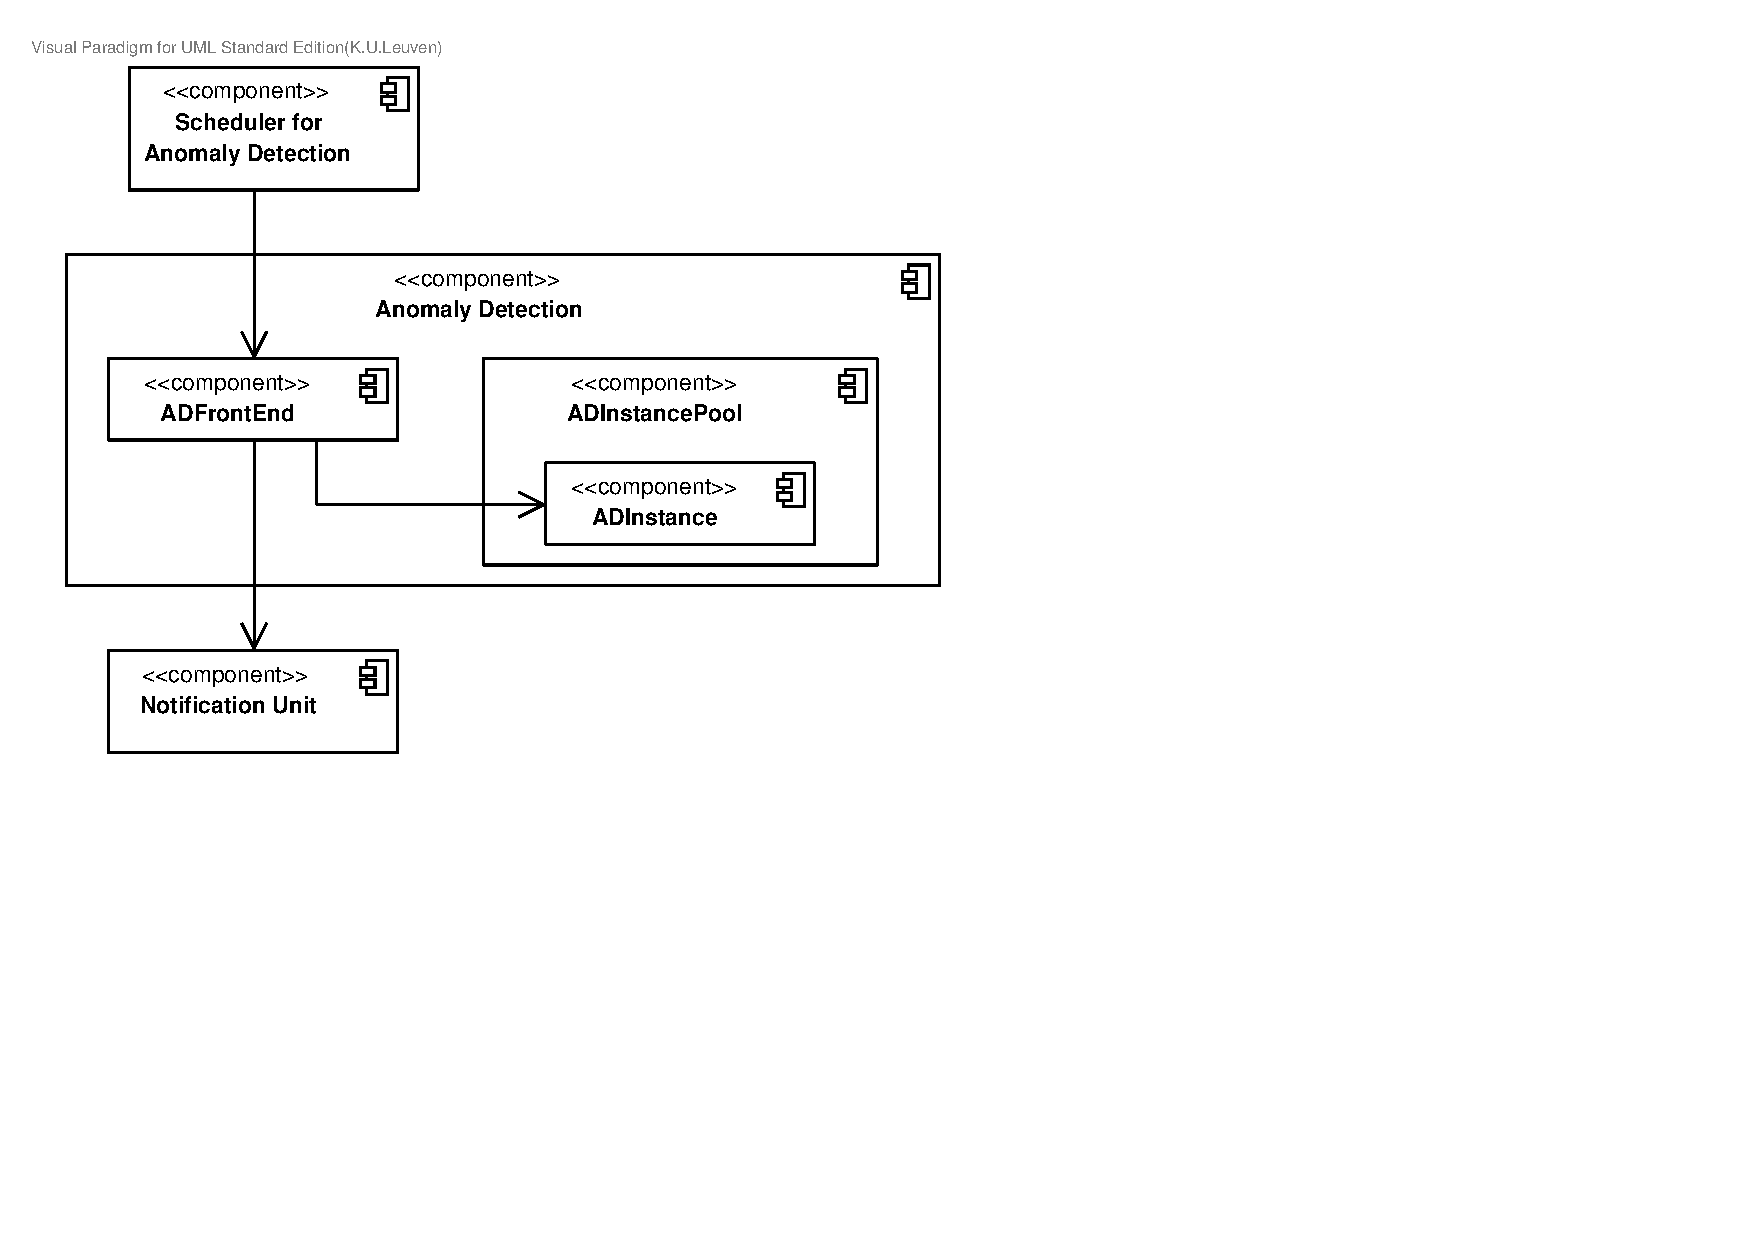
\includegraphics[width=\textwidth]{figs/add-it6-elements.pdf}
		\caption{Overview of all instantiated child elements in the Anomaly
		Detection Unit.}
		\label{fig:it6/elements}
	\end{centering}
\end{figure}

\subsection{Step 4: Define interfaces for instantiated elements}
\label{add:it6/interfaces}

\npar In this section each interface is explained in terms of the components
which use and/or offer it together with information about what is exchanged. For
detailed information with reference to the specific methods the interfaces
implement, we refer to the interface catalog, see appendix
\ref{chap:interface-catalog}.

\subsubsection{AnomalyDetectionAPI}

\npar This interface was already discussed in iteration 1, see
\ref{add:it1/interfaces}.

\subsubsection{ADInstancePoolAPI}

\npar The \interface{ADInstancePoolAPI} lies in between the ADFrontEnd and the
ADInstancePool. Through this interface are ADInstances exchanged.

\subsubsection{ADInstanceAPI}

\npar The ADInstance offers an interface towards its user (i.e. the ADFrontEnd)
where results of anomaly detection algorithms are passed through.

\npar On overview of all the components and their interfaces is shown in figure
\ref{fig:it6/interfaces}.

\begin{figure}[H]
	\begin{centering}
		% TODO Figure
		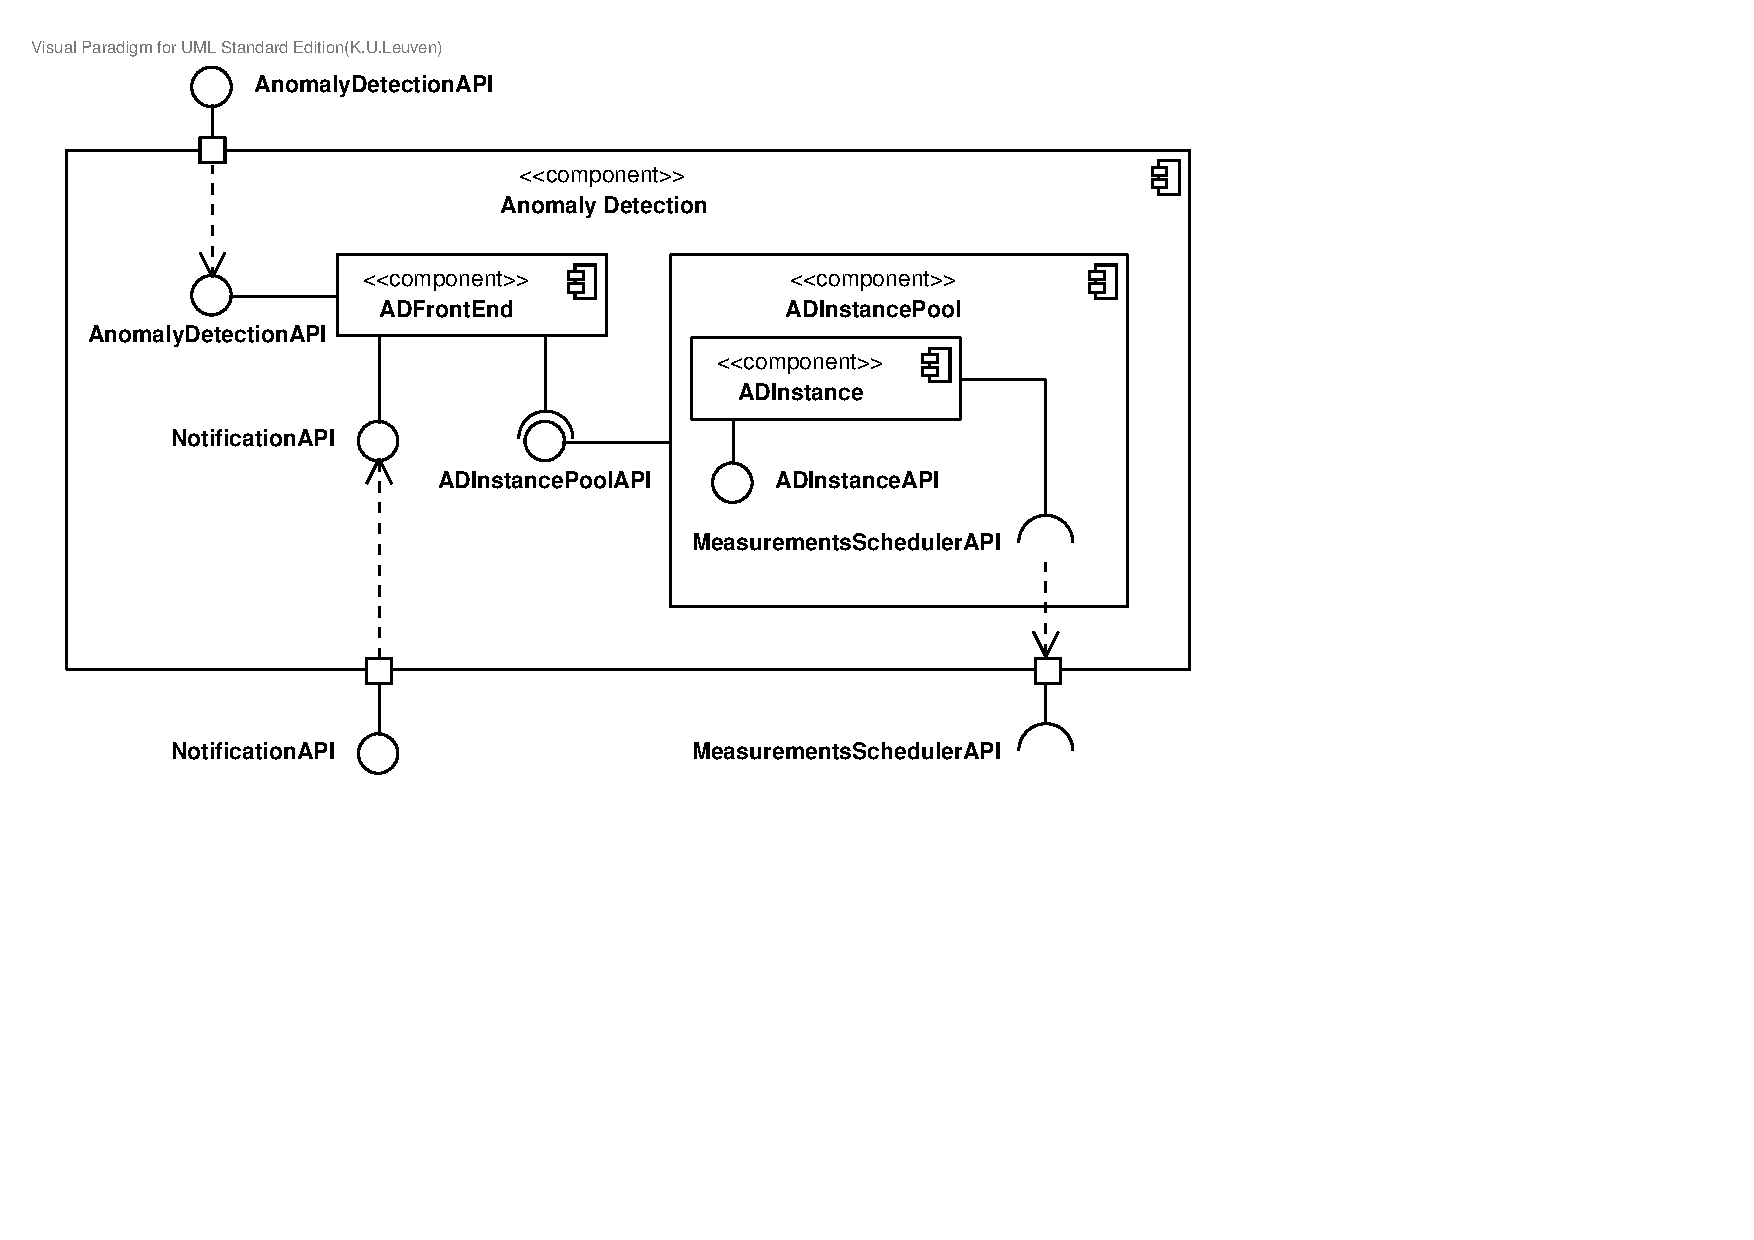
\includegraphics[width=\textwidth]{figs/add-it6-interfaces.pdf}
		\caption{Overview of the interfaces and components in the Anomaly Detection
		Unit.}
		\label{fig:it6/interfaces}
	\end{centering}
\end{figure}

\subsection{Step 5: Verify and refine}
\label{add:it6/verification}

\npar The quality attribute P2' (introduce parallellism) is resolved in this
iteration. The actual anomaly detection (UC10) is delegated to ADInstance.
